\section{Rkmh}

\begin{frame}{Rkmh I}
    \begin{columns} % align columns
        \begin{column}{.60\textwidth}
            \begin{itemize}
                \item Hyperparameter: k-mer-size $ k $, sketch-size $ s $ \pause
                \item Reads und Referenzgenom werden zu k-mers umgewandelt \pause
                \item k-mers werden gehasht \pause
                \item Die Hashs werden sortiert und die ersten $ s $ für den Vergleich genommen \pause
                \item Weitere Reduzierung der Datenmenge durch Bereitstellung von unterschiedliche Filtern \pause
            \end{itemize}
        \end{column}
        \hfill
        \begin{column}{.40\textwidth}
            \begin{figure}[H]
                \centering
                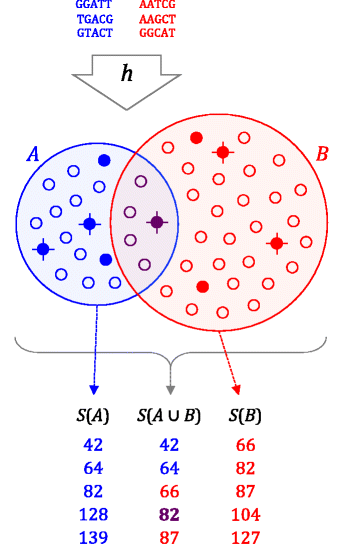
\includegraphics[width=0.85\textwidth]{images/mash_similarity.png} 
                \caption{Reduzierung der Datenmenge über MinHash \cite{mashSimilarityImage}}
            \end{figure}
        \end{column}
    \end{columns}
\end{frame}


\begin{frame}{Rkmh II}
    \begin{itemize}
        \item Beispiel-Filter\footnote{\url{https://github.com/edawson/rkmh}}: 
        \begin{itemize}
            \item --min-kmer-occurence <int>: Entfernt k-mers die nur <int> mal auftreten
            \item --max-samples <int>: Entfernt k-mers die in mehr als <int> Referenzgenomen auftreten
        \end{itemize} \pause
        \item Entwickelt in C++ mit OpenMP \pause
        \item Hash-Funktion: MurMurHash3\footnote{\url{https://github.com/aappleby/smhasher/wiki/MurmurHash3}}
    \end{itemize}
\end{frame}

\begin{frame}{Rkmh III - Ergebnisse}
    \begin{columns} % align columns
        \begin{column}{.45\textwidth}
            \begin{itemize}
                \item Umfassende Tests wurden auf verschiedenen Datensätzen sowie Testdaten\footnotemark[1] durchgeführt \pause
                \item Gute Hyperparameter-Einstellungen sketch-size  $ s \geq 4000 $ k-mer-size $ 10 < k \leq 18 $ \pause
            \end{itemize}
        \end{column}
        \begin{column}{.50\textwidth}
            \begin{figure}[H]
                \centering
                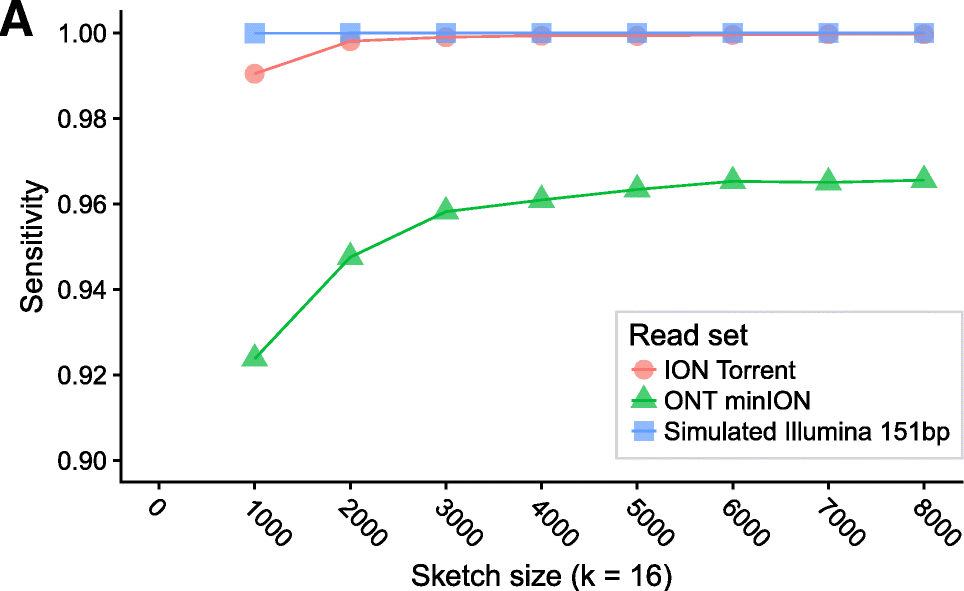
\includegraphics[width=0.85\textwidth]{images/hyper-params-a.png} 
                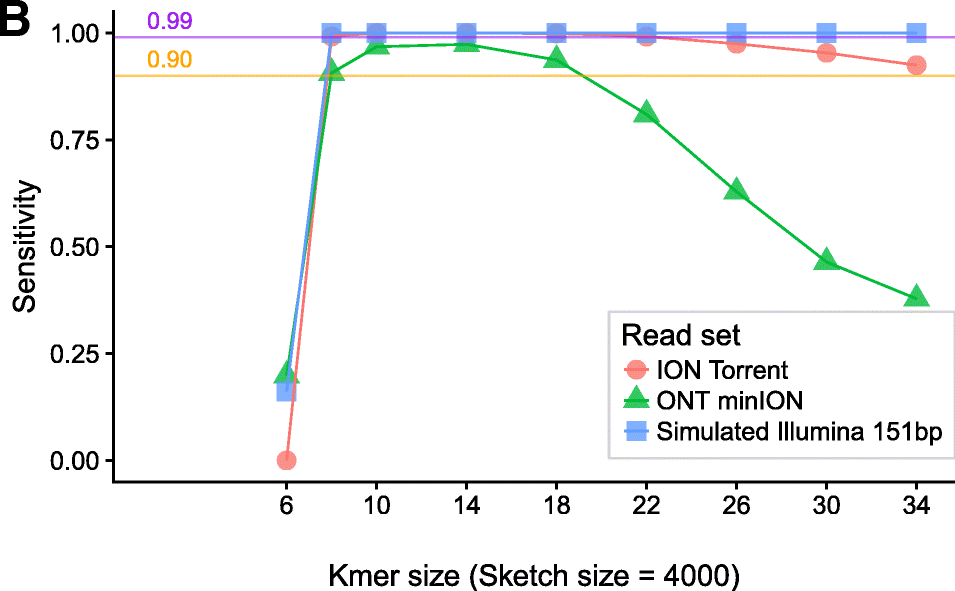
\includegraphics[width=0.85\textwidth]{images/hyper-params-b.png}
                \caption{Ermittlung von optimalem $ s $ und $ k $ \cite{rkmhHyperParamImageA,rkmhHyperParamImageB}}
            \end{figure} 
        \end{column}
    \end{columns}        

    \footnotetext[1]{\url{https://github.com/edawson/rkmh_sim_data}}
\end{frame}